\documentclass{pssbmac}

%%%%%%%%%%%%%%%%%%%%%%%%%%%%%%%%%%%%%%%%%%%%%%%%%%%%%%%%%%%%%%%%%%%%%%%%
%% POR FAVOR, NÃO FAÇA MUDANÇAS NESSE PADRÃO QUE ACARRETEM  EM
%% ALTERAÇÃO NA FORMATAÇÃO FINAL DO TEXTO
%%%%%%%%%%%%%%%%%%%%%%%%%%%%%%%%%%%%%%%%%%%%%%%%%%%%%%%%%%%%%%%%%%%%%%%%

%%%%%%%%%%%%%%%%%%%%%%%%%%%%%%%%%%%%%%%%%%%%%%%%%%%%%%%%%%%%%%%%%%%%%%%%
% POR FAVOR, ESCOLHA CONFORME O CASO
%%%%%%%%%%%%%%%%%%%%%%%%%%%%%%%%%%%%%%%%%%%%%%%%%%%%%%%%%%%%%%%%%%%%%%%%
\usepackage[brazilian]{babel} % texto em Português
%\usepackage[english]{babel} % texto em Inglês

%\usepackage[latin1]{inputenc} % acentuação em Português ISO-8859-1
\usepackage[utf8]{inputenc} % acentuação em Português UTF-8
%%%%%%%%%%%%%%%%%%%%%%%%%%%%%%%%%%%%%%%%%%%%%%%%%%%%%%%%%%%%%%%%%%%%%%%%

%%%%%%%%%%%%%%%%%%%%%%%%%%%%%%%%%%%%%%%%%%%%%%%%%%%%%%%%%%%%%%%%%%%%%%%%
%% POR FAVOR, NÃO ALTERAR
%%%%%%%%%%%%%%%%%%%%%%%%%%%%%%%%%%%%%%%%%%%%%%%%%%%%%%%%%%%%%%%%%%%%%%%%
\usepackage[T1]{fontenc}
\usepackage{float}
\usepackage{graphics}
\usepackage{graphicx}
\usepackage{epsfig}
\usepackage{indentfirst}
\usepackage{amsmath, amsfonts, amssymb, amsthm}
\usepackage{url}
\usepackage{csquotes}
% Ambientes pré-definidos
\newtheorem{theorem}{Theorem}[section]
\newtheorem{lemma}{Lemma}[section]
\newtheorem{proposition}{Proposition}[section]
\newtheorem{definition}{Definition}[section]
\newtheorem{remark}{Remark}[section]
\newtheorem{corollary}{Corollary}[section]
\newtheorem{teorema}{Teorema}[section]
\newtheorem{lema}{Lema}[section]
\newtheorem{prop}{Proposi\c{c}\~ao}[section]
\newtheorem{defi}{Defini\c{c}\~ao}[section]
\newtheorem{obs}{Observa\c{c}\~ao}[section]
\newtheorem{cor}{Corol\'ario}[section]

% ref bibliográficas
\usepackage[backend=biber, style=numeric-comp, maxnames=50]{biblatex}
\addbibresource{refs.bib}
\DeclareTextFontCommand{\emph}{\boldmath\bfseries}
\DefineBibliographyStrings{brazil}{phdthesis = {Tese de doutorado}}
\DefineBibliographyStrings{brazil}{mathesis = {Disserta\c{c}\~{a}o de mestrado}}
\DefineBibliographyStrings{english}{mathesis = {Master dissertation}}
%%%%%%%%%%%%%%%%%%%%%%%%%%%%%%%%%%%%%%%%%%%%%%%%%%%%%%%%%%%%%%%%%%%%%%%%


\begin{document}

%%%%%%%%%%%%%%%%%%%%%%%%%%%%%%%%%%%%%%%%%%%%%%%%%%%%%%%%%%%%%%%%%%%%%%%%
% TÍTULO E AUTORAS(ES)
%%%%%%%%%%%%%%%%%%%%%%%%%%%%%%%%%%%%%%%%%%%%%%%%%%%%%%%%%%%%%%%%%%%%%%%%

\title{Análise visual de alguns erros de ponto flutuante e de Units of Last Place em experimentos computacionais}

\author{
    {\large Ribas, E. R. L. D.}\thanks{enzorochaeleitedinizribas@gmail.com}\\
    {\large D'Afonseca, L. A.}\thanks{autor3@email}  \\
    {\large Rocha, L. M.}\thanks{autor3@email}  \\
    {\small DM/CEFET-MG, Belo Horizonte, MG} \\
}
\criartitulo
%%%%%%%%%%%%%%%%%%%%%%%%%%%%%%%%%%%%%%%%%%%%%%%%%%%%%%%%%%%%%%%%%%%%%%%%
%%%%%%%%%%%%%%%%%%%%%%%%%%%%%%%%%%%%%%%%%%%%%%%%%%%%%%%%%%%%%%%%%%%%%%%%
% TEXTO
%%%%%%%%%%%%%%%%%%%%%%%%%%%%%%%%%%%%%%%%%%%%%%%%%%%%%%%%%%%%%%%%%%%%%%%%
Este trabalho apresenta resultados de estudos realizados em um projeto de iniciação científica cujo objetivo é explorar graficamente alguns efeitos do cálculos realizados com ponto flutuante e das Unidades de Última Posição (Units of Last Place - ULP).

Um sistema de ponto flutuante (SPF) é a maneira utilizada pelos computadores para representar números reais através de uma notação compacta e eficaz. Ele permite escrever números de grandezas diversas utilizando apenas números inteiros. No entanto, essa representação fica limitada ao adequar o número ao sistema adotado, causando erros que podem se acumular em operações sucessivas, produzindo resultados imprecisos ou incorretos.

O \cite{IEEE754} é um padrão para a representação de números em ponto flutuante em sistemas computacionais, que define formatos de precisão simples (32 bits) e dupla (64 bits). Ele especifica como os números devem ser representados, incluindo a forma como os bits são alocados para o sinal, o expoente e a mantissa.

O número representado em ponto flutuante em computadores é então calculado como:

\vspace{-.3cm}
\begin{equation}
x = (-1)^s \times (1 + \sum_{i=1}^{t-1} (d_i \times \beta^{-i})) \times \beta^e,
\end{equation}
onde $s$ é o bit de sinal, $d_i$ são os dígitos significativos, $e$ é o expoente, $\beta$ é a base e $t$ é o número de dígitos significativos. O expoente é armazenado com um viés, ou seja, o valor real do expoente é calculado como $e = E - bias$, onde $E$ é o valor armazenado e $bias$ é um valor constante que depende do formato  utilizado. O sistema para 64 bits, utilizado na maioria dos computadores atuais, é definido por $\beta = 2$, $t = 53$, $L = -1022$ e $U = 1023$.

A Unit of Last Place (ULP) é a menor diferença entre dois números representáveis em ponto flutuante, ou seja, a distância entre um número e o próximo número representável, \cite{muller2005}.
A natureza discreta do sistema de ponto flutuante junto a limitação de casas decimais da mantissa impactam na precisão de um sistema de ponto flutuante. O conjunto de números se torna mais esparso quanto mais distante o número for de zero, aumentando o erro relativo. Dessa forma a ULP se torna uma medida relativa importante para avaliar a precisão dos cálculos realizados com ponto flutuante, podendo ser calculada como:
\begin{equation}
ULP(x) = \beta^{e_x - t + 1},
\label{eq:ulp}
\end{equation}
\vspace{-1cm}
\begin{figure}[H]
\centering
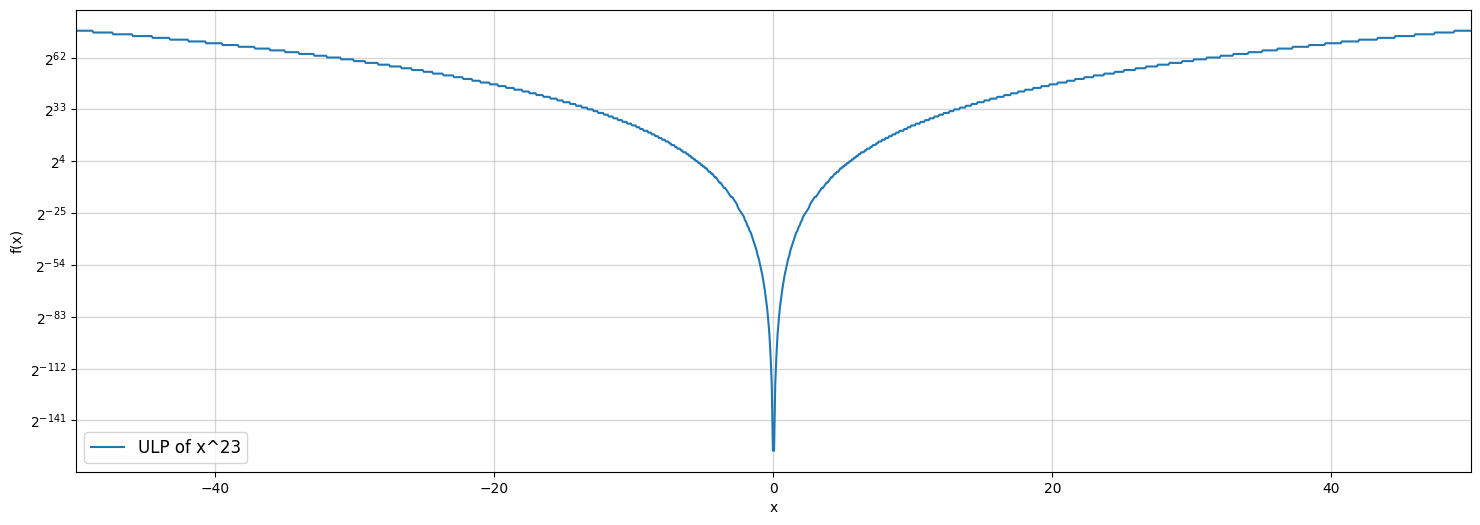
\includegraphics[width=.8\textwidth]{images/ulp.png}
\caption{ {\small Gráfico da Função $ULP(x^{23})$. Fonte: Autor.}}
\label{fig:ulp}
\end{figure}
\vspace{-1.5cm}

Um erro comum em SPF's é o da perda de significância, ou cancelamento catastrófico, que ocorre quando a subtração de dois números resulta em um valor com menos dígitos significativos do que os números originais.
Um exemplo desse comportamento é a função $f(x) = x^{10} + l - x^{10}$. Embora para $x \in \mathbb{R}$ o resultado é igual a $l$, ao efetuarmos os cálculos usando ponto flutuante, observamos o comportamento ilustrado no gráfico da figura \ref{fig:numError1}, em que o valor correto é exibido apenas até um certo valor de $x$. Após esse valor observamos um intervalo em que ocorre uma oscilação caótica no resultado da função. Posteriormente, observamos que a função assume o valor zero.
\begin{figure}[H]
\centering

\includegraphics[width=.8\textwidth]{images/NumError1_mplt}
\caption{ {\small Cancelamento Catastrófico. Fonte: Autor.}}
\label{fig:numError1}
\end{figure}
Essa oscilação é conjecturada a ser relacionada diretamente com a $ULP(x)$ no intervalo em que ela ocorre. Como ilustrado nas figuras \ref{fig:ulp_f} e \ref{fig:ulp_f_overlapped}, a função $f(x)$ e a $ULP(x)$ se tornam próximas no intervalo em que ocorre a oscilação, sugerindo que o erro relativo da função $f(x)$ é da está associado diretamente a $ULP(x)$ nesse intervalo.
\begin{figure}[H]
\centering
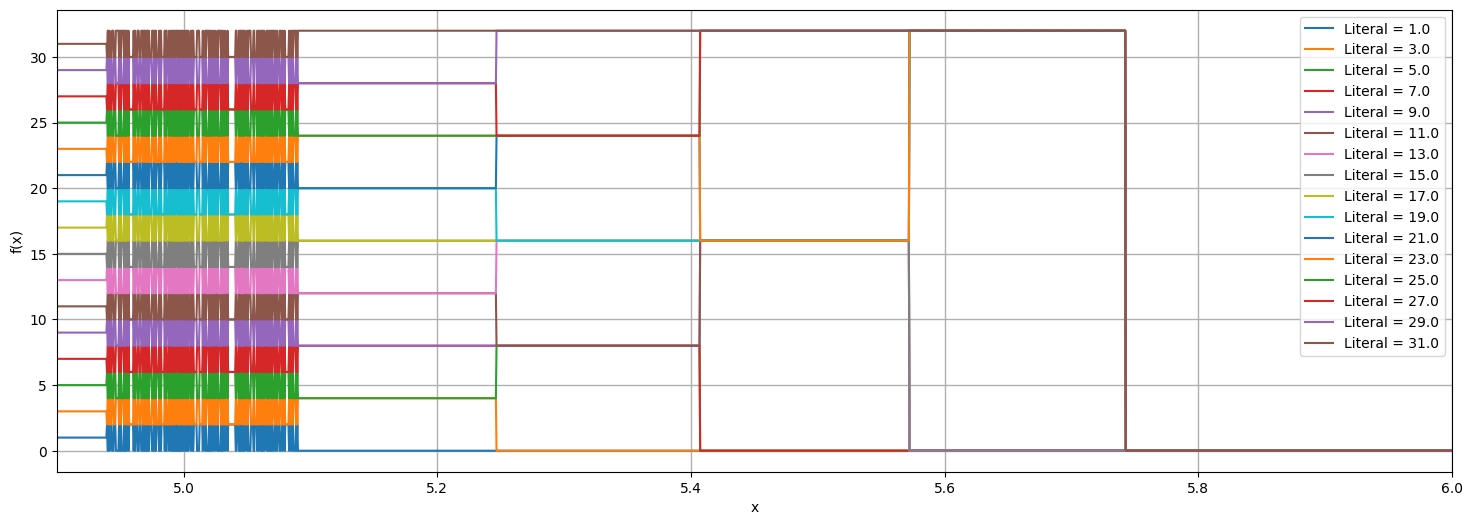
\includegraphics[width=.8\textwidth]{images/errors1.png}
\caption{ {\small Cancelamento Catastrófico para $l$ variando de 1 a 32 com passo 2. Fonte: Autor.}}
\label{fig:erros1}
\end{figure}

\begin{figure}[H]
\centering
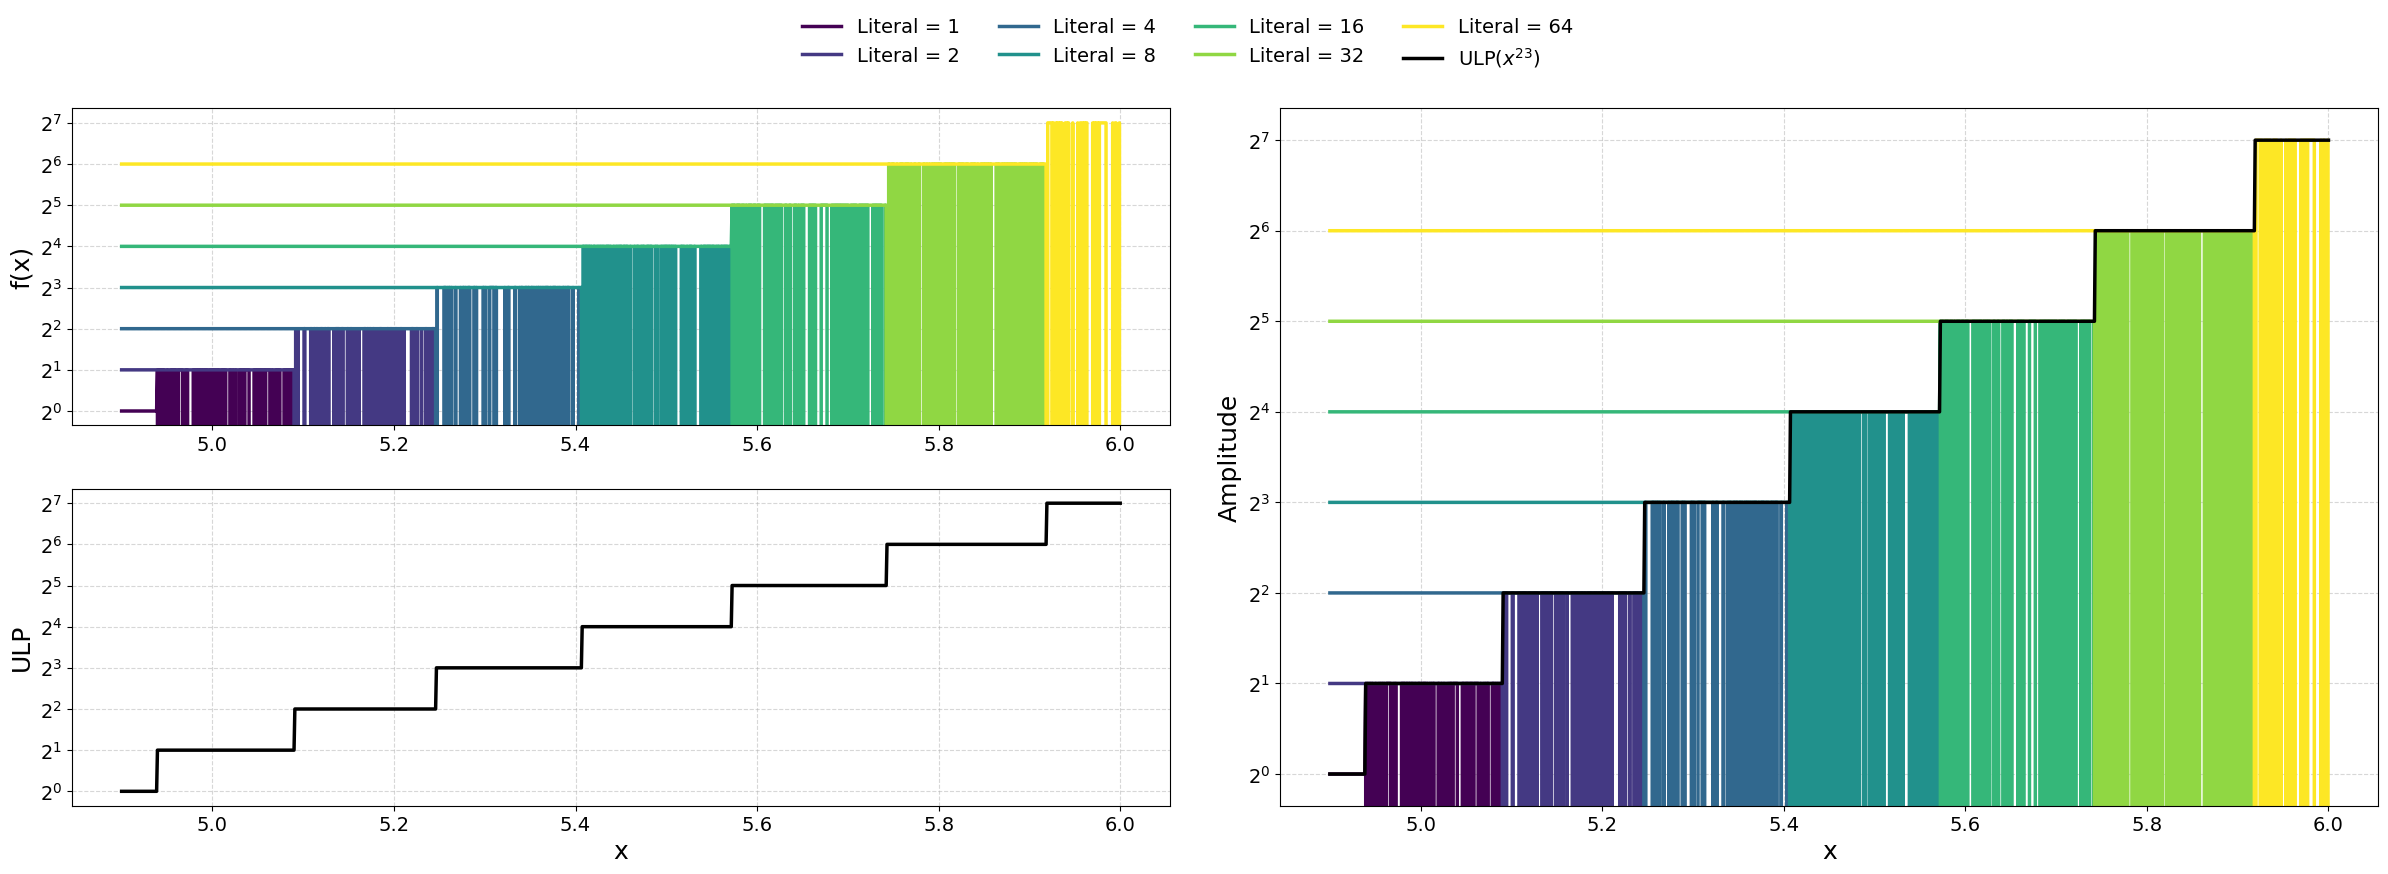
\includegraphics[width=1\textwidth]{images/errors_and_ulp3.png}
\caption{ {\small Cancelamento Catastrófico comparado com a ULP. Fonte: Autor.}}
\label{fig:ulp_f}
\end{figure}

TINHA ESSAS IMAGENS ABAIXO TAMBÉM, MAS PREFERI AS OUTRAS
\begin{figure}[H]
\centering
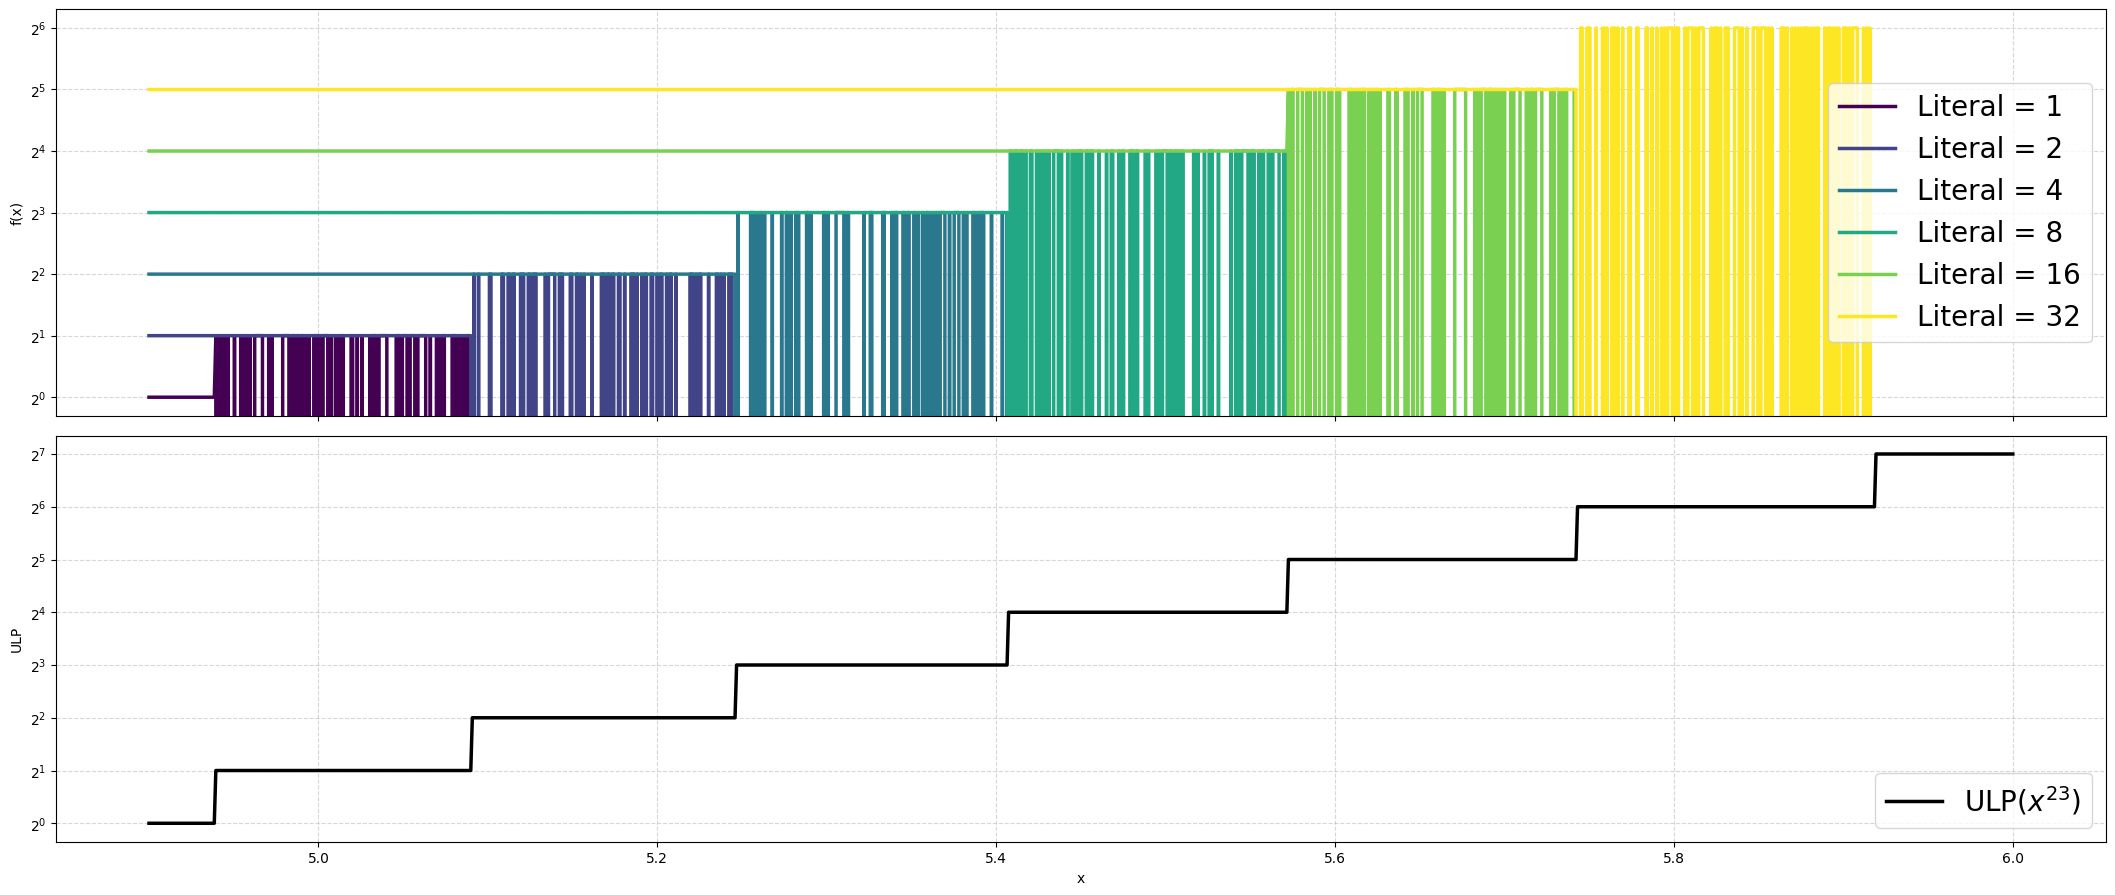
\includegraphics[width=.5\textwidth]{images/ulp_and_errors.png}
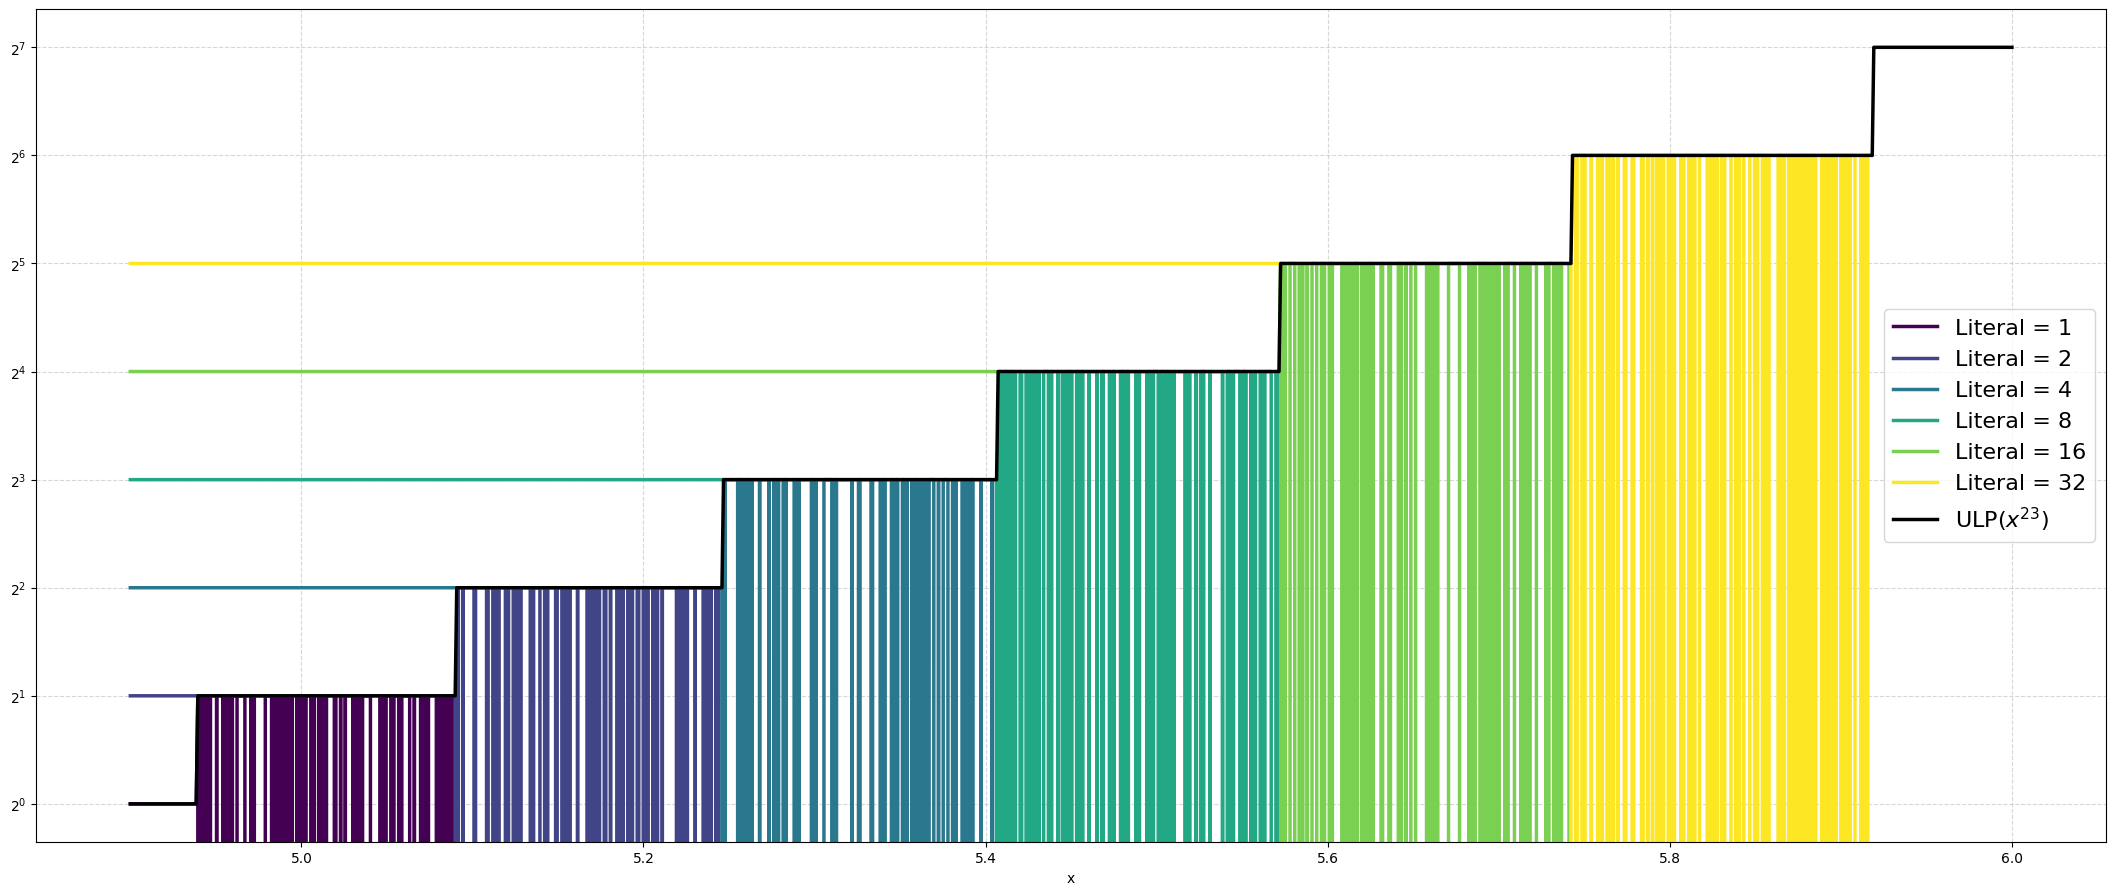
\includegraphics[width=.5\textwidth]{images/ulp_and_errors2.png}
\caption{ {\small Ulp Lado a lado com a função $f(x)$. Fonte: Autor.}}
\label{fig:ulp_f}
\end{figure}

\begin{figure}[H]
\centering
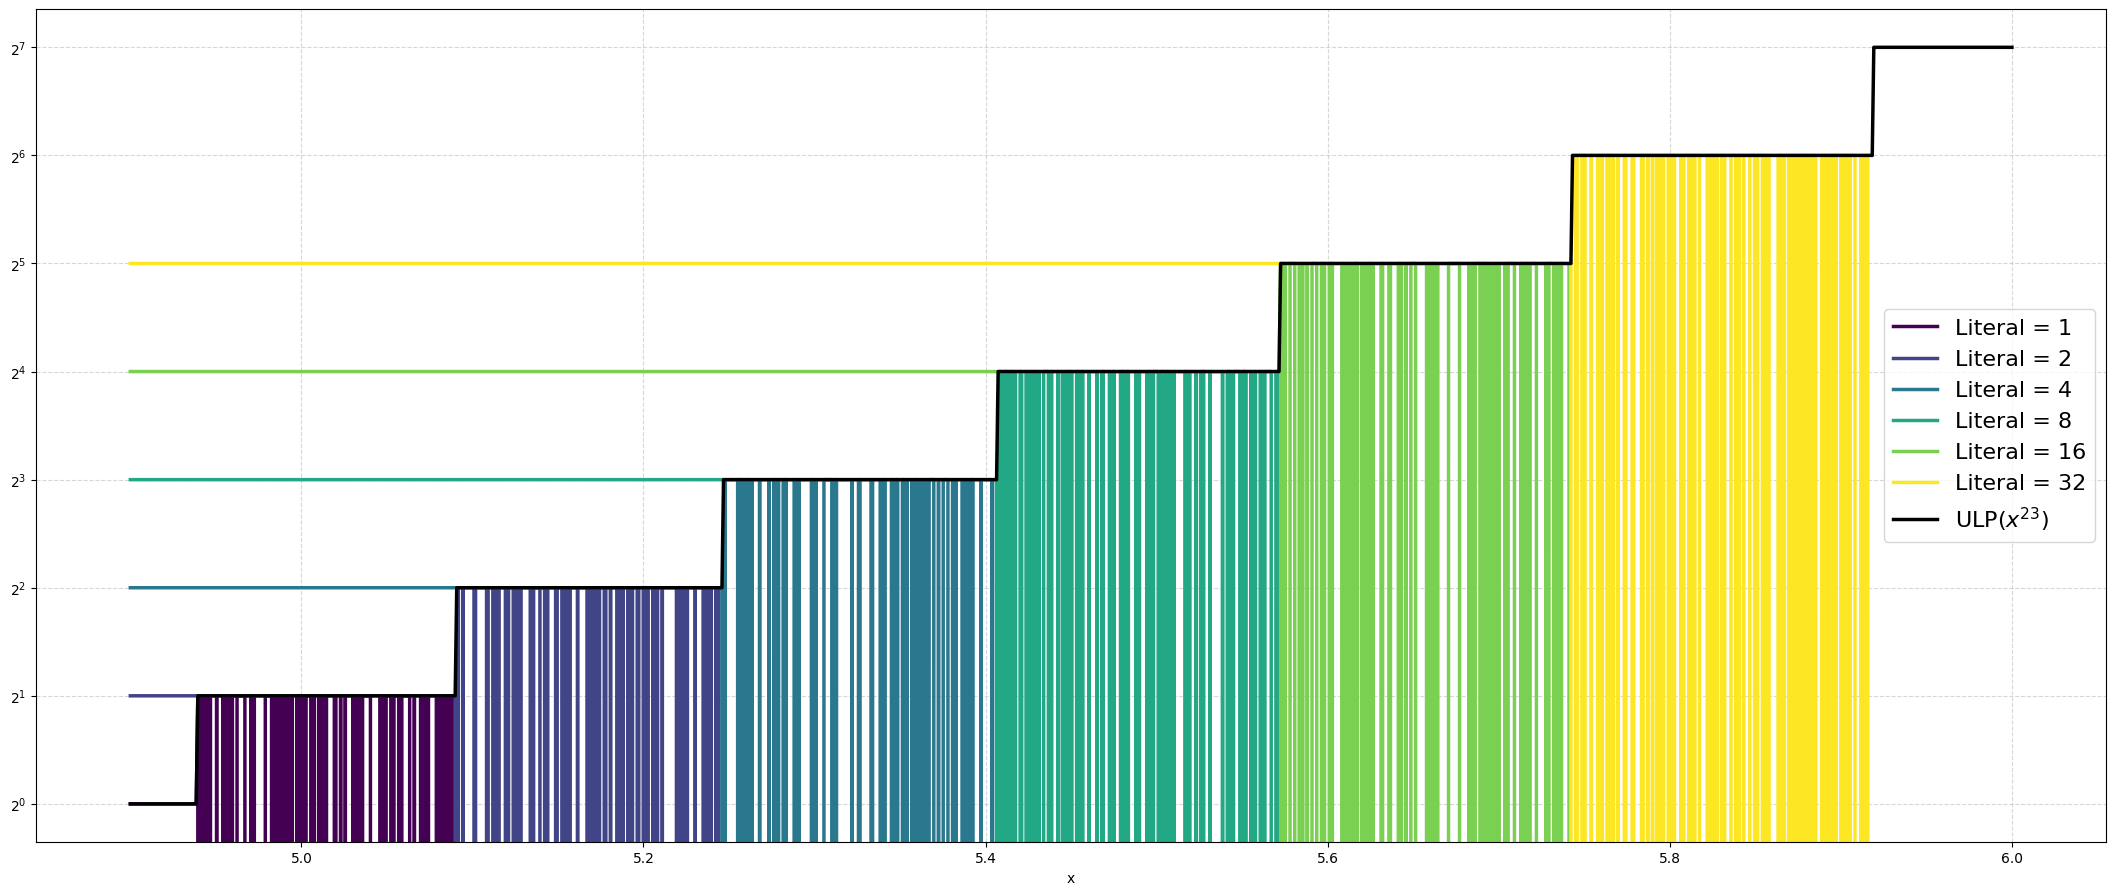
\includegraphics[width=.5\textwidth]{images/ulp_and_errors2.png}
\caption{ {\small $Ulp(x)$ sobreposto com a função $f(x)$. Fonte: Autor.}}
\label{fig:ulp_f_overlapped}
\end{figure}



%%%%%%%%%%%%%%%%%%%%%%%%%%%%%%%%%%%%%%%%%%%%%%%%%%%%%%%%%%%%%%%%%%%%%%%%
% REFS BIBLIOGRÁFICAS
% POR FAVOR, NÃO ALTERAR
%%%%%%%%%%%%%%%%%%%%%%%%%%%%%%%%%%%%%%%%%%%%%%%%%%%%%%%%%%%%%%%%%%%%%%%%
\nocite{*}
\printbibliography
%%%%%%%%%%%%%%%%%%%%%%%%%%%%%%%%%%%%%%%%%%%%%%%%%%%%%%%%%%%%%%%%%%%%%%%%

\end{document}




